\section{Использование высокопроизводительных вычислительных систем}

\subsection{Вычислительные системы}
Одним из наиболее интересных направлений развития современной вычислительной
техники являются многопроцессорные системы. В настоящее время происходит фантастически
быстрый рост мощности
вычислительной техники, что дает реальную возможность
приступить к моделированию тех задач, которые ранее были недоступны для
численного решения. Но, с другой стороны, пришлось столкнуться с той ситуацией,
когда высокопроизводительная многопроцессорная вычислительная техника используется 
лишь на небольшую часть своих потенциальных возможностей. Эта проблема в первую очередь 
связана с трудностями адаптации алгоритмов решения к архитектуре многопроцессорных 
ЭВМ с распределенной памятью. 
 
Многопроцессорные системы можно разделить на 2 класса - системы с общей памятью
и системы с распределенной памятью.
\begin{enumerate}
\item  Системы с общей памятью. 

С точки зрения программиста привлекательно выглядят системы с общей памятью.
Разбитая на взаимодействующие процессы (нити) программа в большинстве таких
систем автоматически распределяется по доступным процессорам системы. Достаточно
широкий круг последовательных алгоритмов может быть успешно адаптирован к
функционированию на системах с общей, или, что тоже самое, разделяемой памятью.

Однако у систем с общей памятью есть ряд существенных недостатков:
\begin{itemize}
\item относительно небольшое число процессоров;
\item отсутствие возможности наращивания числа процессоров - масштабируемости;
\item пиковая производительность систем с общей памятью ниже пиковой
производительности систем с раздельной памятью;
\item высокая, относительно аналогичных по производительности систем с
раздельной памятью, стоимость.
\end{itemize}
Сказанное выше приводит к тому, что сконструированная система, как правило, не
предусматривает возможности существенного наращивания числа процессорных узлов и
обуславливает крайне высокую, относительно рассматриваемых систем с раздельной
памятью, стоимость.
 
\item Системы с распределенной памятью.
 Масштабируемые системы массового параллелизма конструируют на основе
объединения каналами передачи данных процессорных узлов, обладающих своей
локальной оперативной памятью, недоступной другим процессорам. Обмен данными
между процессорами при таком подходе возможен лишь с помощью сообщений,
передаваемых по каналам связи. Такая схема обладает рядом преимуществ по
сравнению с системами, построенными на основе общей памяти. Подчеркнем основные
преимущества систем с распределенной памятью:
\begin{itemize}
\item сравнительно низкая стоимость;
\item масштабируемость (возможность построения систем требуемой
производительности и наращивания их мощности за счет установки дополнительных
процессоров).
\end{itemize}

Системы с раздельной памятью, по-видимому, всегда будут лидировать по показателю
пиковой производительности, поскольку любые новые однопроцессорные (или
многопроцессорные на основе общей памяти) системы могут быть легко объединены
сетью и использованы в качестве многопроцессорных комплексов с раздельной
памятью. 

Но, к сожалению, эффективное использование систем с распределенной памятью
требует значительных усилий со стороны разработчиков прикладного обеспечения и
возможно далеко не для всех типов задач. Для широкого круга хорошо
зарекомендовавших себя последовательных алгоритмов не удается построить
эффективные параллельные аналоги.
\end{enumerate}

\subsection{О технологии CUDA}
В настоящее время графические процессоры (GPU -- Graphics Processing Unit)
являются оптимальной по соотношению цена-производительность параллельной 
архитектурой с общей памятью. Причина высокой производительности видеокарт 
в том, что они изначально были сконструированы для одновременного применения
одной и той же шейдерной функции к большому числу пикселей, или, другими 
словами, для высокопроизводительных параллельных вычислений.

До недавнего времени использовать вычислительный мощности видеокарт было
крайне неудобно, так как программисту необходимо было
овладеть шейдерным языком программирования, соответствующему коду,
выполняемому на GPU. Причем, в графических API полностью отсутствует
возможность взаимодействия между параллельно обрабатываемыми пикселами,
что в графике действительно не нужно, а для вычислительных задач оказывается довольно
желательным. Ситуация изменилась, когда появились средства разработки
GPGPU-приложений(General-Purpose computing on Graphics Processing Units). 
В качестве таких средств выступают CUDA, OpenCL, Dx11 Compute
Shaders. 

Предложенная компанией Nvidia технология CUDA (Compute Unified Device Architecture) -- 
заметно облегчает написание GPGPU-приложений. Данная технология предназначена для
разработки приложений для массивно-параллельных вычислений. Все программы пишутся на
<<расширенном>> языке C, есть хорошая документация, инструменты, набор библиотек,
поддерживается кроссплатформенность. CUDA является полностью бесплатной и уже 
приобрела широкую популярность в научных кругах~\cite{Boreskov}.

CUDA строится на концепции, что GPU выступает в роли массивно-параллельного
сопроцессора к CPU. При этом последовательный код выполняется на CPU,
а для массивно-параллельных вычислений соответствующий код выполняется на
GPU как набор одновременно выполняющихся нитей(потоков, threads).

Таким образом, GPU рассматривается как специализированное вычислительное устройство,
которое:
\begin{enumerate}
  \item является сопроцессором к CPU;
  \item обладает собственной памятью;
  \item обладает возможностью параллельного выполнения огромного количества отдельных
  нитей.
\end{enumerate}

В данной работе рассматривается применение технологии CUDA к задачам 
трехфазной фильтрации. Портирование кода происходило на базе
примеров из ~\cite{Sanders-CUDA}.

\subsection{Параллелизм}

В данной работе в основу параллельной реализации положен принцип геометрического параллелизма.
Геометрический параллелизм является одним из наиболее распространенных типов
параллелизма, применяемых при решении задач, где имеется большое число
однородных действий над однородными данными, которые можно так разбить на
группы, что при обработке каждой группы не потребуется обращений к данным из
других групп, за исключением их малого числа.
Последнее свойство будем называть свойством локальности алгоритма. Локальный
алгоритм допускает разбиение данных на части по числу процессоров, при котором
обработку каждой части осуществляет соответствующий процессор. Этот подход
весьма эффективен при условии, что действия, выполняемые одним процессором,
зависят лишь от небольшого, ограниченного объема данных, расположенных на других
процессорах. Желательно, чтобы эти <<чужие>> данные были локализованы на
ограниченном, небольшом количестве процессоров.
В настоящее время широкое распространение получил стандарт разработки
параллельных программ MPI (Message Passing Interface - интерфейс передачи
сообщений) для систем с разделенной памятью. 
В данной работе он используется для осуществления передачи
сообщений между процессорами.

\subsection{Практические аспекты реализации программного комплекса}

\subsubsection*{Программный комплекс}
Программный комплекс написан на языке
программирования С/C++ с использованием с помощью средств
библиотек MPI и CUDA в среде Eclipse CDT. Комплекс является
кроссплатформенным и запускается как в системах Windows и Linux, что
позволяет использовать его на различных кластерах и пользовательских ПК.

\subsubsection*{Индексация массива данных}
Для однородности способа обращения к данным независимо
от размерности задачи используется одномерная индексация массивов.
Например, обращение к элементу $T(i,j,k)$:
$T[i + j * locN_x + k * locN_x * locN_y]$.
$locN_x, locN_y, locN_z$ -- размеры расчетной сетки, обрабатываемой
данным процессором. Продемонстируем универсальность данного
подхода. Допустим, отсутствует измерение, соответвующее $z$, тогда
$locN_z=1$, $k$ <<пробегает>> значения от $0$ до $locN_z-1$, т.е.
в данном случае единственное возможное значение $k=0$, при этом
обращение к элементу становится идентичным $T[i + j * locN_x]$, т.е.
двумерной индексации. Таким образом, учет размерности задачи
происходит автоматически. Однако, в коде при вычислении,
например, градиента функции следует все же проверять, что $locN_z > 2$
(если используется трехточечный шаблон),
прежде чем проводить вычисления.

\subsubsection*{Сетка из процессоров}
Расчетная область делится на подобласти в одном, двух или трех направлениях.
Можно сказать, что процесоры образуют сетку, в которой
местоположение каждого процессора может быть задано с помощью
декартовых координат.
Для наглядности приведем пример такого деления на Рис.~\ref{pic_div}.
\begin{figure}[!h]\center
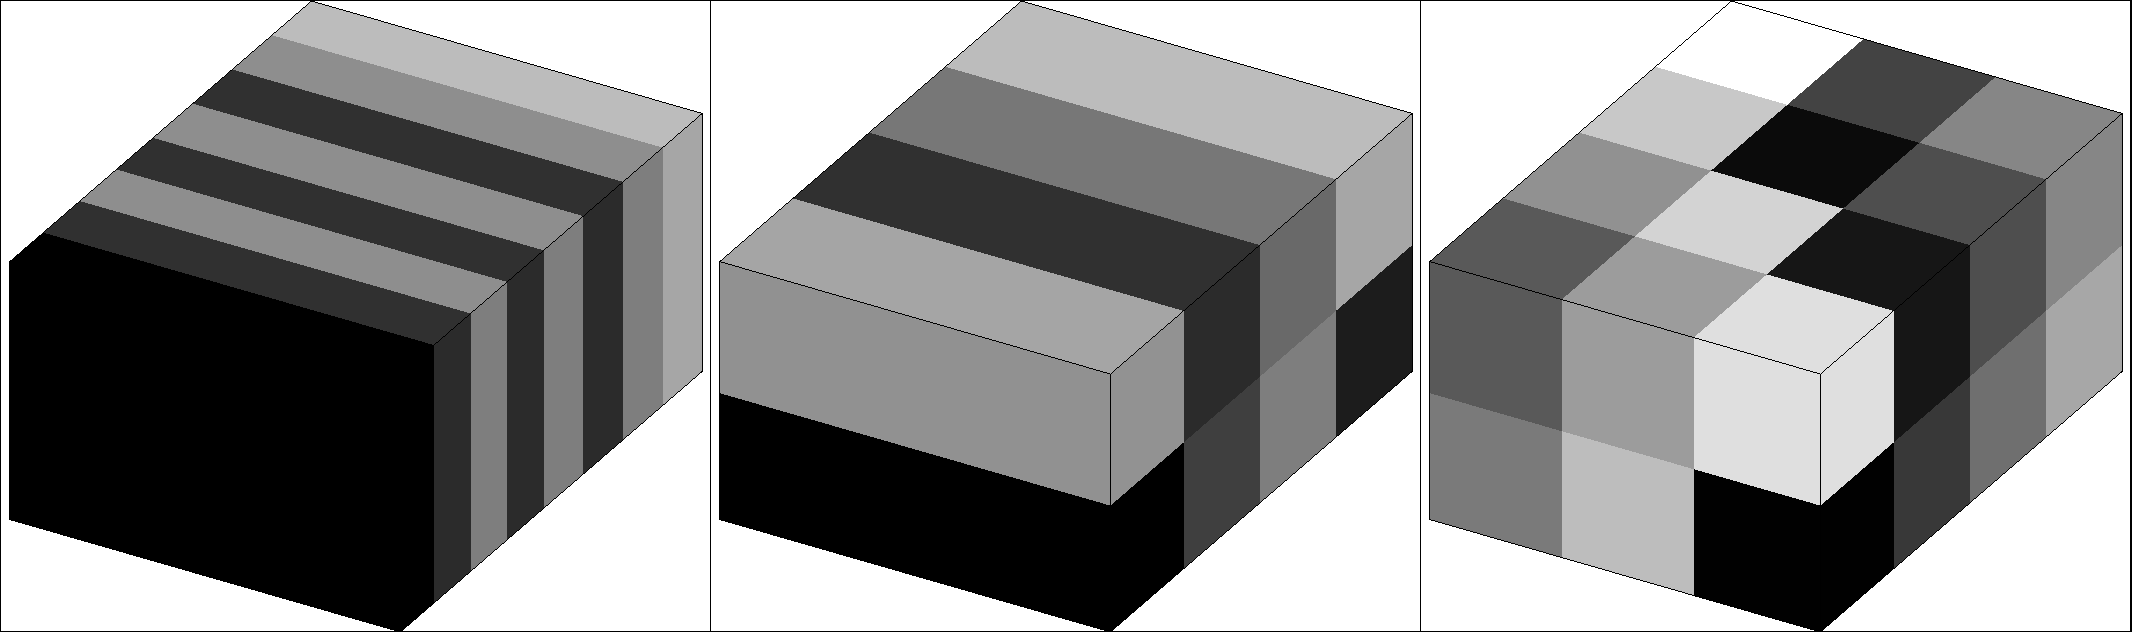
\includegraphics[width=1\textwidth]{div.png} 
\caption{Деление расчетной области на подобласти в одном, двух или трех направлениях}
\label{pic_div}
\end{figure}
Дополнительно к стандартным для MPI понятиям $size$, $rank$
каждым из процессоров запоминаются значения $size_x$, $size_y$, $size_z$,
$rank_x$, $rank_y$, $rank_z$ (аналоги $size$, $rank$ отдельно для каждого из направлений).
$size_x$, $size_y$, $size_z$ определяются алгоритмом деления,
причем $size_x \cdot size_y \cdot size_z = size$.
Ранги определяются в Листинге~\ref{lst_ranks}, причем
$rank_x + rank_y \cdot size_x + rank_z \cdot size_x \cdot size_y = rank$.
\begin{listing}
\begin{minted}[bgcolor=bg, fontfamily=helvetica]{c}
rankx = rank % sizex;
ranky = (rank / sizex) % sizey;
rankz = (rank / sizex) / sizey;
\end{minted}
\caption{Определение координат процессора}
\label{lst_ranks}
\end{listing}
Данные обозначения вводятся для удобства реализации обменов
данными и обращения к расчетной области.

\subsubsection*{Алгоритм первоначального распределения области по процессорам}

Для того чтобы предварительно оценить время, необходимое для расчета, выяснить, насколько 
рационально деление области по различным измерениям, и эффективно распределить нагрузку
между вычислительными узлами, был разработан и встроен в основной код программы
алгоритм первоначального распределения области по процессорам.

В случае многопроцессорной реализации в общем времени вычислений можно выделить
три основных составляющих: время непосредственно численного расчета, время
межпроцессорных обменов и время загрузки/выгрузки данных на графический ускоритель 
(в случае гибридных вычислительных систем). Доля, которую вносит каждое из
слагаемых, зависит как от вычислительной системы, так и от выбора конфигурации разбиения
области. Чем больше направлений разбиения, тем меньше граничных узлов, но
больше количество обменов на границах.

Предлагаемый алгоритм автоматического выбора оптимального разбиения состоит
из трех основных шагов:
\begin{enumerate}
 \item Найти эмпирически время, идущее на вычисления в одной расчетной точке на
одном временном слое задачи. Следует заметить, что нахождение времени расчета
аналитически в одной точке не является тривиальной задачей, а экспериментально засечь
время расчета можно только для некоторого множества точек на нескольких слоях по
времени. Для разного числа точек получаем набор времен и строим зависимость времени
расчета некоторого числа точек от их количества. Для явных схем эту зависимость
можно приближенно считать линейной. В этом случае имеет смысл говорить о времени
расчета одной точки. Для неявных схем зависимость нелинейна, с увеличением числа
точек растет время, условно приходящееся на расчет значения в одной точке.
\item Найти эмпирически время, идущее на коммуникации. Для нахождения времени
пересылки между CPU, принадлежащими разным узлам кластера, измеряются времена
пересылок для различного объема данных. Предполагается, что время пересылки
состоит из времени инициализации соединения и времени непосредственно 
отправки-получения данных, которое линейно зависит от объема данных. Из полученных 
измерений можно найти данную линейную зависимость. Время копирования данных из памяти
CPU в память GPU определяется аналогичным способом.
\item Решить задачу поиска минимума общего времени вычислений при ограниченном
числе доступных вычислителей. Эту задачу можно решить, перебрав в цикле все возможные
способы разбиения области при заданном количестве расчетных точек.
\end{enumerate}
Рассмотрим пример применения данного алгоритма. Допустим, что нужно произвести
расчеты на трехмерной сетке размером $500\times100\times50=2.5$ млн точек, при этом в
распоряжении пользователя имеется 24 ядра CPU. Можно оценить, насколько сильно
меняется общее время вычислений в зависимости от того, каким образом распределена
расчетная сетка. На Рис.~\ref{diagr_div} представлены результаты измерений полученных времен 
расчета некоторой тестовой задачи трехфазного просачивания для различных конфигураций разбиения.
Видно, что времена вычислений могут отличаться как на пять процентов,
так и в полтора раза, что может быть очень существенно.

\begin{figure}
\begin{center}
\begin{tikzpicture}
  \begin{axis}[ymax=35, ymin=0, ybar, enlarge x limits=true, width=0.6\textwidth, x label style={below=10mm},
    xlabel={конфигурация $(size_x\ size_y \ size_z)$}, ylabel={время расчета, с},
    symbolic x coords={(3 4 2),(24 1 1),(12 2 1),(6 4 1),(8 2 2),(4 3 2),(2 6 2)},
    xtick=data,nodes near coords, nodes near coords align={vertical}, x tick label style={rotate=45,anchor=east},]
     \addplot coordinates {((3 4 2),19.8) ((24 1 1),29.7) ((12 2 1),26.55) ((6 4 1),20.81) ((8 2 2),20.3) ((4 3 2),19.98) ((2 6 2),19.91)};
  \end{axis}
\end{tikzpicture}
\caption{Времена расчета тестовой задачи для различных конфигураций для 24 процессоров}
\label{diagr_div}
\end{center}
\end{figure}

\subsubsection*{Локальная и глобальная системы координат}
В работе представлен гибкий и хорошо масштабируемый механизм разделения
расчетной сетки на локальные подсетки. Благодаря такому механизму
нет необходимости хранить расчетную сетку целиком на каком-либо из
процессоров, а преобразование локальных координат к глобальным
позволяет воссоздать общую картину полученных в результате расчетов
данных.
Используем следующие обозначения:
$locN_x, locN_y, locN_z$ -- размеры расчетной сетки, обрабатываемой
данным процессором (локальной), $N_x, N_y, N_z$ -- размеры общей (глобальной) сетки.
Разделение глобальной сетки на локальные происходит с помощью
алгоритма, описанного в Листинге~\ref{lst_globallocal}. 
Если сетка по выделенному измерению поровну не делится, то процессоры с $rank_x < N_x \% size_x$ получают нагрузку
на один слой больше. Каждый процессор содержит дополнительный слой в массиве для обмена данными, при 
наличии <<соседа>> (если есть <<соседи>> с обеих сторон -- два дополнительных слоя).
Глобальные границы хранятся как обычные точки.

Переход от локальной
системы координат к глобальной представлен в Листинге~\ref{lst_localglobal}.

\begin{listing}
\begin{minted}[bgcolor=bg, fontfamily=helvetica]{c}
locNx = Nx / sizex;
if (rankx < Nx % sizex) locNx++;
if (sizex > 1) {
    if ((rankx == 0) || (rankx == sizex - 1)) locNx++;
    else locNx += 2;
}
locNy = Ny / sizey;
if ((ranky < Ny % sizey)) locNy++;
if (sizey > 1) {
    if ((ranky == 0) || (ranky == sizey - 1)) locNy++;
    else locNy += 2;
}
locNz = Nz / sizez;
if (rankz < Nz % sizez) locNz++;
if (sizez > 1) {
    if ((rankz == 0) || (rankz == sizez - 1)) locNz++;
    else locNz += 2;
}
\end{minted}
\caption{Разделение расчетной сетки на подсетки}
\label{lst_globallocal}
\end{listing}

\begin{listing}
\begin{minted}[bgcolor=bg, fontfamily=helvetica]{c}
int global_index = local_index;
switch (axis)
{
case 'x':
    global_index += rankx * (Nx / sizex) + min(rankx, Nx % sizex) - min(rankx, 1);
    break;
case 'y':
    global_index += ranky * (Ny / sizey) + min(ranky, Ny % sizey) - min(ranky, 1);
    break;
case 'z':
    global_index += rankz * (Nz / sizez) + min(rankz, Nz % sizez) - min(rankz, 1);
    break;
default:
    print_error();
}
return global_index;
\end{minted}
\caption{Переход от локальной системы координат к глобальной}
\label{lst_localglobal}
\end{listing}

\subsubsection*{Организация межпроцессорных обменов}

В первую очередь граничные данные для обмена помещаются
буферный массив. Затем посредством сообщений процессоры
обмениваются содержимым буферов. Процессоры условно делятся
на четные и нечетные отдельно по всем трем направлениям пересылки.
По каждому направлению процессоры обмениваются в два этапа:
от четных к нечетным и от нечетных к четным. Таким образом,
полный обмен граничными данными со всеми <<соседями>> происходит
за шесть итераций. Реализация обменов описанным способом 
приводится в Листингах~\ref{lst_exchange}, \ref{lst_exchanges}. 
Обмен завершается копированием
полученных данных из буфера в локальную расчетную область процессора.

При проведении расчетов на GPU к обмену сообщениями и использованию
буфера на хосте
добавляется копирование данных для обмена из памяти видеокарты
в память хоста.

\begin{listing}
\begin{minted}[bgcolor=bg, fontfamily=helvetica]{c}
void send_recv(double* arr, char axis, double* buf, int size, int dst_rank, int id) {
  MPI_Status status;
  load_exchange_data_part(arr, axis);
  MPI_Sendrecv_replace(buf, size, MPI_DOUBLE, dst_rank, id, dst_rank, id + 1,
		       MPI_COMM_WORLD, &status);
  save_exchange_data_part(arr, axis);
}
void recv_send(double* arr, char axis, double* buf, int size, int dst_rank, int id) {
  MPI_Status status;
  load_exchange_data_part(arr, axis);
  MPI_Sendrecv_replace(buf, size, MPI_DOUBLE, dst_rank, id + 1, dst_rank, id,
		       MPI_COMM_WORLD, &status);
  save_exchange_data_part(arr, axis);
}
\end{minted}
\caption{Реализация межпроцессорного двустороннего обмена}
\label{lst_exchange}
\end{listing}
\begin{listing}
\begin{minted}[bgcolor=bg, fontfamily=helvetica]{c}
void exchange_direct(double* arr, char axis, double* buf) {
  switch(axis) {
  case 'x': if(sizex > 1) {
    if (rankx % 2 == 0) {
      if (rankx != sizex - 1) send_recv(arr, axis, buf, locNy * locNz, rank + 1, 500);
      if (rankx != 0) recv_send(arr, axis, buf, locNy * locNz, rank - 1, 502);
    } else {
      if (rankx != 0) recv_send(arr, axis, buf, locNy * locNz, rank - 1, 500);
      if (rank) != sizex - 1) send_recv(arr, axis, buf, locNy * locNz, rank + 1, 502);
    }
  } break;
  case 'y': if(sizey > 1) {
    if (ranky % 2 == 0) {
      if (ranky != sizey - 1) send_recv(arr, axis, buf, locNx * locNz, rank + sizex, 504);
      if (ranky != 0) recv_send(arr, axis, buf, locNx * locNz, rank - sizex, 506);
    } else {
      if (ranky != 0) recv_send(arr, axis, buf, locNx * locNz, rank - sizex, 504);
      if (ranky != sizey - 1) send_recv(arr, axis, buf, locNx * locNz, rank + sizex, 506);
    }
  } break;
  case 'z': if(sizez > 1) {
    if (rankz % 2 == 0) {
      if (rankz != sizez - 1)
	send_recv(arr, axis, buf, locNx * locNy, rank + sizex * sizey, 508);
      if (rankz != 0) recv_send(arr, axis, buf, locNx * locNy, rank - sizex * sizey, 510);
    } else {
      if (rankz != 0) recv_send(arr, axis, buf, locNx * locNy, rank - sizex * sizey, 508);
      if (rankz != sizez - 1)
	send_recv(arr, axis, buf, locNx * locNy, rank + sizex * sizey, 510);
    }
  } break;
  default: break;
  }
}
\end{minted}
\caption{Организация межпроцессорных пересылок по всем направлениям}
\label{lst_exchanges}
\end{listing}

\subsubsection*{Понятие активной точки}
По способу обработки узлы расчетной сети условно можно
разделить на:
\begin{itemize}
 \item активные (значения в которых вычисляются текущим процессором);
 \item вспомогательные (служащие для хранения данных, полученных от
 других процессоров).
\end{itemize}
Для определения, к какому из типов относится данный узел,
используется код, представленный в Листинге~\ref{lst_act_point}.
\begin{listing}
\begin{minted}[bgcolor=bg, fontfamily=helvetica]{c}
if (((rankx != 0 && i == 0) || (rankx != sizex - 1 && i == locNx - 1 && Nx > 1))
  || ((ranky != 0 && j == 0) || (ranky != sizey - 1 && j == locNy - 1 && Ny > 1))
  || ((rankz != 0 && k == 0) || (rankz != sizez - 1 && k == locNz - 1 && Nz > 1)))
    return 0;
else
    return 1;
\end{minted}
\caption{Определение типа расчетного узла}
\label{lst_act_point}
\end{listing}

\subsubsection*{Ввод/Вывод данных}
Сохранение данных занимает важное место в моделировании
физических процессов. Как отмечено в \cite{Yakobovsky},
ввод и вывод исходных данных с внешних дисковых накопителей может осуществляться, как минимум,
двумя разными способами:
\begin{itemize}
\item ввод/вывод данных выполняет один из процессоров, называемый в
дальнейшем <<управляющий>>;
\item ввод/вывод данных выполняется непосредственно каждым процессором.
\end{itemize}
Несмотря на болльшую универсальность первого способа,
выбран второй способ, так как он является более подходящим
в случае обработки данных, объем которых превышает оперативную память управляющего
процессорного узла.
В этом случае возможны также, по крайней мере, два варианта:
\begin{itemize}
\item запись всеми процессорами одного большого файла -- каждый процессор
пишет свой фрагмент этого файла;
\item запись каждым процессором отдельного файла -- общее число файлов
при этом соответствует числу процессоров.
\end{itemize}
Для лучшей масштабируемости системы, удобства визуализации и обращения
к данным выбран первый способ,
но при этом возникает проблема синхронизации доступа к файлу.
Приведем пример кода, обеспечивающего корректную запись данных в файл
многими процессорами в Листинге~\ref{lst_print_plot}.
\begin{listing}
\begin{minted}[bgcolor=bg, fontfamily=helvetica]{c}
for (int cpux = 0; cpux < sizex; cpux ++)
    for (int i = 0; i < Nx / sizex + 3; i++)
	for (int cpuy = 0; cpuy < sizey; cpuy ++)
	    for (int j = 0; j < def.Ny / sizey + 3; j++)
		for (int cpuz = 0; cpuz < sizez; cpuz ++)
		{
		    barrier();
		    if ((rank == cpux + cpuy * sizex + cpuz * sizex * sizey)
			  && (i < locNx) && (j < locNy))
		    {
			for (int k = 0; k < locNz; k++)
			    if (is_active_point(i, j, k))
				print_plot_row(i, j, k);
		    }
		}
\end{minted}
\caption{Синхронизация вывода в файл между процессорами}
\label{lst_print_plot}
\end{listing}

\subsection{Результаты расчетов на кластере}

Основные расчеты проводились на кластере К-100, ИПМ им. М.В.Келдыша РАН, 
структура которого изображена на Рис~\ref{pic_k100}.
Ускорения и эффективность вычислений
были подробно проанализированы на примере тестовой задачи 1, описанной в соответствующем
разделе. 

\begin{figure}[!h]\center
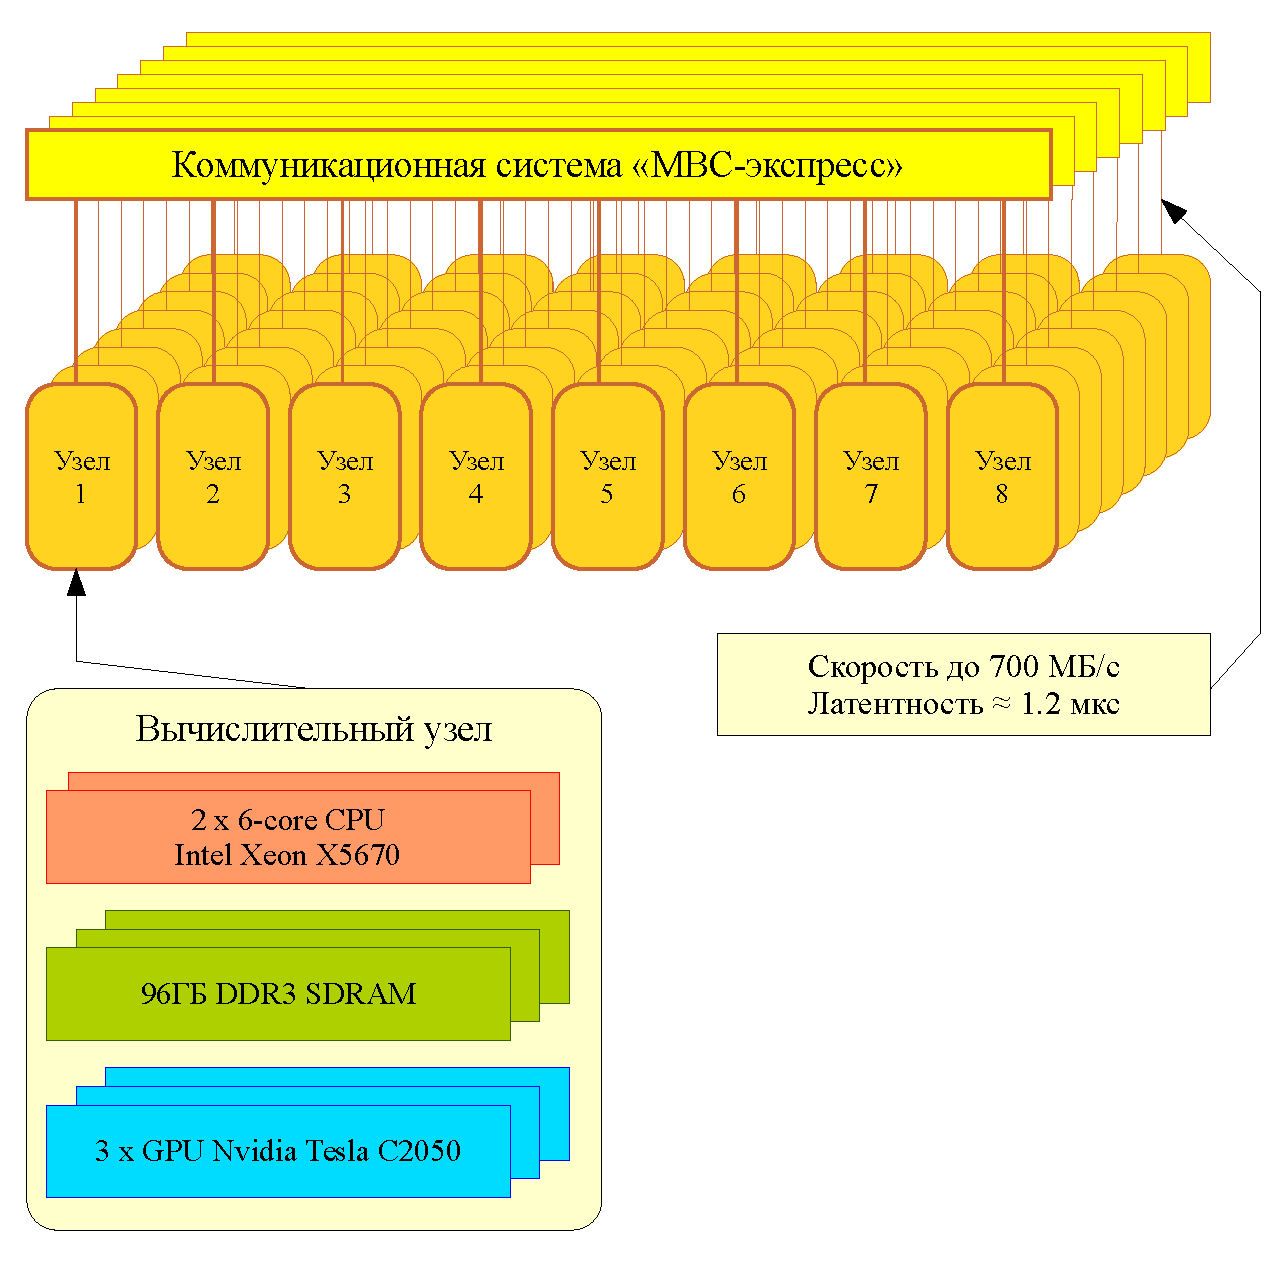
\includegraphics[width=0.8\textwidth]{k100.pdf} 
\caption{Структура гибридного кластера К100}
\label{pic_k100}
\end{figure}

\subsubsection*{Результаты применения библиотеки MPI}

На приведенных графиках (Рис.~\ref{mpi_speedup}, Рис.~\ref{mpi_eff}) изображены
ускорения и эффективности вычислений в зависимости от числа расчетных узов сетки для 
различного числа процессоров.
Измерялось время расчета 50 шагов по времени на сетке размером 4 миллиона узлов
с помощью счетчика, встроенного в программный код.
Расчетная область может быть поделена между CPU геометрически как в одном, так в двух и трех направлениях.
Ступенчатая структура ускорений и, следовательно, скачки эффективности наблюдаются
в связи с неодинаковым способом распределения нагрузки между процессорами
в зависимости от их числа, а также погрешностью вычислений. Сохранение высокой
эффективности вычислений (84-95\%) обусловлено значительным превосходством времени, требуемого
непосредственно для расчета, по сравнению с временем, необходимым для обмена данными
между процессорами.

\begin{figure}
\begin{center}
\begin{tikzpicture}
  \begin{axis}[axis lines=left, enlargelimits=true, grid=major, width=0.7\textwidth, xlabel={\textit{число процессоров}}, ylabel={\textit{ускорение}}]
    \pgfplotstableread{data/mpi_times.txt}{\mytable}
    \pgfplotstablegetelem{0}{Y}\of{\mytable}
    \pgfmathsetmacro{\ay}{\pgfplotsretval}
    \addplot [blue, mark=*] table [x=X, y expr=\ay/\thisrow{Y}] {\mytable};
  \end{axis}
\end{tikzpicture}
\caption{Зависимость ускорения расчета тестовой задачи от числа процессоров}
\label{mpi_speedup}
\end{center}
\end{figure}

\begin{figure}
\begin{center}
\begin{tikzpicture}
  \begin{axis}[axis lines=left, enlargelimits=true, grid=major, width=0.7\textwidth, xlabel={\textit{число процессоров}}, ylabel={\textit{эффективность}}]
    \pgfplotstableread{data/mpi_times.txt}{\mytable}
    \pgfplotstablegetelem{0}{Y}\of{\mytable}
    \pgfmathsetmacro{\ay}{\pgfplotsretval}
    \addplot [blue,mark=*] table [x=X, y expr=\ay/\thisrow{Y}/\thisrow{X}] {\mytable};
  \end{axis}
\end{tikzpicture}
\caption{Зависимость эффективности расчета тестовой задачи от числа процессоров}
\label{mpi_eff}
\end{center}
\end{figure}


\subsubsection*{Результаты совместного применения библиотек CUDA и MPI}


